\documentclass{report}

\input{../templates/preamble}
\input{../templates/macros}
\input{../templates/letterfonts}

\title{\Huge{Electon Self Energy Corrections}}
\author{\Huge{Marcus Allen Denslow}}
\date{2026-01-09}

\begin{document}

\maketitle
\newpage% or \cleardoublepage
% \pdfbookmark[<level>]{<title>}{<dest>}
\pdfbookmark[section]{\contentsname}{toc}
\tableofcontents
\pagebreak

If one calculates the energy of a point charge using classical electromagnitism, the result is infinate, yet as far as we know, the electron is point charge. One can calculate the energy needed to assemble an electron due, essentially, to the interaction of the electron with its own field. A uniform charge distribution with the classical radius of an electron, we have an energy $\displaystyle m_{e}c^2$. Experiments have probed the electron's charge distribution and found that it is consistent with a point charge down to distances much smallen than the classical radius. Beyond classical calculations, the self energy of the electron calculated in the quantum theory of Dirac is still infinate but the divergences are less severe. 
\\
At this pint we must take the unpleasant position (constant) infinate energy should just be subtracted when we consider the overall zero of energy (as we did for the field energy in the vacuum). Electrons exist and don't carry infinate amount of energy baggage so we just subtract off the infinate constant. Nevertheless, we will find that the electron's self energy may change when it is a bound state and we should account for this change in out energy level calculations. This calculation will also give us the opportunity to understand resonant behaviour in scattering.
\\
We can calculate the lowest order self energy corrections represented by the two Feynman diagrams below.

\begin{figure}[h!]
    \centering
    % First diagram (a)
    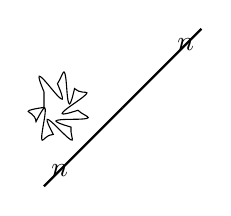
\begin{tikzpicture}[scale=1]
        % Left diagram
        % Lines
        \draw[thick] (-1,-1) -- (0,0);
        \draw[thick] (0,0) -- (1,1);
        % Wavy loop
        \draw[decorate, decoration={coil, aspect=0, segment length=2mm, amplitude=2mm}] (-1,0.2) .. controls (-0.5,0.5) and (-0.5,-0.5) .. (-1,-0.2) -- cycle;
        % Labels
        \node at (-0.8,-0.8) {$n$};
        \node at (0.8,0.8) {$n$};
    \end{tikzpicture}
    \hspace{2cm}
    % Second diagram (b)
    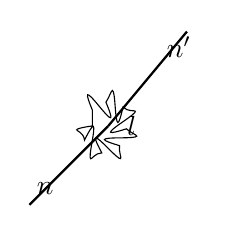
\begin{tikzpicture}[scale=1]
        % Lines
        \draw[thick] (-1,-1) -- (0,0);
        \draw[thick] (0,0) -- (1,1.2);
        % Wavy loop connected to slanted line
        \draw[decorate, decoration={coil, aspect=0, segment length=2mm, amplitude=2mm}] (-0.2,0.2) .. controls (0.3,0.5) and (0.3,-0.5) .. (-0.2,-0.2) -- cycle;
        % Labels
        \node at (-0.8,-0.8) {$n$};
        \node at (0.9,1.0) {$n'$};
        \node at (0.3,0) {$l$};
    \end{tikzpicture}

    \vspace{1em}

    \noindent (a) \hspace{5cm} (b)
\end{figure}



\end{document}
